\documentclass[11pt]{article}

% --- packages ---
\usepackage[utf8]{inputenc}
\usepackage[T1]{fontenc}
\usepackage[margin=1in]{geometry}
\usepackage{booktabs}
\usepackage{graphicx}
\usepackage{amsmath}
\usepackage{siunitx}
\usepackage{xcolor}
\usepackage[hidelinks]{hyperref}
\usepackage{natbib}

\sisetup{detect-weight=true, detect-family=true}
\newcommand{\dropneg}[1]{\textcolor{red}{$-#1$}}

\title{PhishRewrite: Measuring the Fragility of Content-Based\\
Phishing Detectors under LLM Rewriting}
\author{%
  Gaurang Katyal\\
  \normalsize Independent Researcher\\
  \normalsize ORCID: \href{https://orcid.org/0009-0001-0850-1673}{0009-0001-0850-1673}%
}
\date{2026}

\begin{document}
\maketitle

\begin{abstract}
Content-based phishing and spam detectors classify an email from its text. We ask
how robust that decision is when an attacker uses a large language model (LLM) to
\emph{rewrite} a phishing email so it reads as more benign while preserving the
malicious ask and all URLs verbatim. We release \textbf{PhishRewrite}, a benchmark
of \num{4000} LLM rewrites of held-out phishing emails at four escalating
severities (from light paraphrase to a full rewrite that keeps only the
call-to-action), generated with two independent model families (Claude Haiku 4.5
and Google Gemini 2.5 Flash), together with the \num{28201}-email labelled corpus
and the verbatim attack prompts. On a strict, label-validity-checked evaluation set
($n=270$) we find that classical bag-of-words detectors degrade measurably under
the attack: a logistic-regression detector's phishing recall falls
12.2 points ($0.989\!\to\!0.867$; McNemar $p=\num{2.1e-9}$) with URLs intact,
and the drop roughly doubles to 22.2 points once the frozen URL feature is
removed---so the URL-intact curve is a \emph{lower bound} on a URL-mutating
attacker. A fine-tuned DistilBERT resists the attack on this phishing corpus, but
the same transformer degrades significantly on an independent, same-era spam
corpus (CEAS-2008), so neural robustness here is \textbf{corpus-dependent} rather
than a general property. Finally, the degradation is a fixable
training-distribution gap: adversarial training on rewrites recovers---and
exceeds---clean detection, and crucially the recovery \emph{generalizes across
rewriting models} (detectors trained only on Haiku rewrites recover detection on
held-out Gemini rewrites, and vice versa). All data, code, and prompts are released
(defanged) under permissive licences for defensive research.
\end{abstract}

\section{Introduction}
Email remains a primary vector for credential theft and fraud, and a large body of
deployed defences rests on \emph{content-based} classification: features extracted
from an email's text decide whether it is phishing. Such detectors are attractive
because they are cheap, interpretable, and do not require reputation or
infrastructure signals. But they make a strong implicit assumption---that the
adversary cannot cheaply rewrite the \emph{surface form} of a malicious message
without abandoning its malicious intent.

Large language models break that assumption. An attacker can now ask an LLM to
rephrase a phishing email---soften its urgency, professionalise its tone,
restructure its sentences---while explicitly instructing it to preserve the
call-to-action and the destination URL. The result is a message that is still
operationally phishing (same ask, same link) but lexically far from the training
distribution a content detector learned.

We quantify exactly how much this matters. Our contributions are:
\begin{enumerate}
  \item \textbf{A benchmark and methodology.} PhishRewrite pairs a labelled corpus
  with \num{4000} LLM rewrites at four severities, a verbatim, committed set of
  attack prompts, and an automated \emph{label-validity contract} that verifies each
  rewrite still carries the malicious ask and its URLs. The headline metric is the
  detector degradation curve versus rewrite severity, on a fixed evaluation set with
  bootstrap confidence intervals.
  \item \textbf{A fragility result with an honest lower bound.} Classical detectors
  degrade under rewriting; the linear model is the most fragile. Because we freeze
  URLs verbatim (to keep the label valid and the URL feature comparable), the
  URL-intact curve understates a real attacker---we show the degradation roughly
  doubles once the frozen URL signal is removed.
  \item \textbf{A corpus-dependence finding for transformers.} A fine-tuned
  DistilBERT resists the attack on the phishing corpus but degrades on an
  independent same-era spam corpus, so we explicitly decline to claim transformers
  are robust in general.
  \item \textbf{A mitigation that generalizes across generators.} Adversarial
  training on rewrites restores detection to (or above) clean levels, and the
  recovery transfers to a rewriting model the detector never trained on.
\end{enumerate}

All artifacts are released defanged for defensive use; see \S\ref{sec:ethics}.

\section{Related Work}
Content-based spam and phishing filtering has a long history, from early Bayesian
filters to modern learned classifiers \citep{sahami1998bayesian}. Adversarial
examples---small input perturbations that flip a classifier's
decision---were formalised for vision \citep{goodfellow2015explaining} and have
analogues in text. Transformer language models \citep{vaswani2017attention,
devlin2019bert} and their distilled variants \citep{sanh2019distilbert} now serve
both as detectors and, in our setting, as the attacker that rewrites the input.
PhishRewrite differs from generic adversarial-text work in two ways: the
perturbation is a \emph{semantically faithful rewrite} produced by an LLM under an
explicit intent-preservation constraint, and we measure detector degradation on a
realistic, label-validity-checked corpus rather than on synthetic token edits.
This study is the email-detection counterpart of a parallel finding in social bot
detection, where account-history (behavioural) features were shown to resist
LLM-driven manipulation that defeats content-based classifiers
\citep{katyal2026bots}: there the robust signal is behavioural; here it is the URL,
and removing it (\S\ref{sec:results}) deepens the collapse.

\section{Threat Model and Attack}\label{sec:method}
\paragraph{Threat model.} The attacker possesses a phishing email and black-box
access to an instruction-following LLM. The goal is to evade a content-based
detector while preserving the malicious function of the email: the
call-to-action (credential entry, payment, link click) and the destination URL(s)
must survive. The attacker does \emph{not} mutate URLs, change infrastructure, or
target a specific deployed detector; this is a deliberately conservative threat
model that yields a lower bound on real-world evasion.

\paragraph{Severity levels.} Each phishing email is rewritten at four escalating,
cumulative severities, defined by committed natural-language instructions:
\begin{itemize}
  \item \textbf{0.25} --- light lexical paraphrase (synonyms, minor wording).
  \item \textbf{0.50} --- $+$ sentence restructuring.
  \item \textbf{0.75} --- $+$ tone/register shift; remove urgency and pressure cues.
  \item \textbf{1.00} --- full rewrite preserving only the ask and the URLs.
\end{itemize}
Severity is rewrite \emph{aggressiveness}, applied to every sampled email; sample
composition is held fixed so only intensity varies along the curve.

\paragraph{Label-validity contract.} A rewrite is a valid adversarial example only
if it preserves the malicious ask and its URL(s). We enforce a \emph{strict}
all-URLs check (every original URL must survive) as the headline contract, and
report a less conservative \emph{primary-URL} variant (only the ask-bearing URL
must survive) as a sensitivity bound. Rewrites that fail are dropped and logged;
the headline degradation curve is computed on the \emph{intersection set}---the
emails whose rewrites pass at all four severities---so $n$ is constant across the
curve. We additionally manually spot-checked a stratified sample of pairs to
confirm the contract.

\section{Experimental Setup}\label{sec:setup}
\paragraph{Corpus.} We assemble \num{28201} emails under a unified schema from
named public research corpora: phishing from the Nazario corpus
\citep{nazario}; ham from the Apache SpamAssassin public corpus
\citep{spamassassin} (ham subsets only) and the Enron corpus
\citep{klimt2004enron}. Generic SpamAssassin spam is excluded to avoid label
noise. The natural class balance is roughly $1\!:\!4.23$ phishing:ham; we do not
resample. Table~\ref{tab:corpus} summarises the split.

\begin{table}[t]
\centering
\caption{Corpus composition and stratified, seeded split.}
\label{tab:corpus}
\begin{tabular}{lrrr}
\toprule
source & phishing (1) & ham (0) & total \\
\midrule
Nazario & \num{5390} & --- & \num{5390} \\
Enron & --- & \num{18700} & \num{18700} \\
SpamAssassin (ham only) & --- & \num{4111} & \num{4111} \\
\midrule
\textbf{total} & \textbf{\num{5390}} & \textbf{\num{22811}} & \textbf{\num{28201}} \\
\bottomrule
\end{tabular}
\\[2pt]
{\footnotesize \num{22560} train / \num{5641} test (stratified, seed 42).}
\end{table}

\paragraph{Detectors and features.} We train three classical detectors---logistic
regression, random forest, and gradient boosting---on TF-IDF features plus
handcrafted signals (length, URL count, urgency-word count, HTML flag, digit and
all-caps ratios, etc.), using scikit-learn \citep{pedregosa2011scikitlearn}. The
TF-IDF vectoriser is fit on train only. We additionally fine-tune
\texttt{distilbert-base-uncased} \citep{sanh2019distilbert} on the same split (head
truncation to 256 tokens; the phishing signal is concentrated early). All
randomness uses a single seed (42).

\paragraph{Attack models.} The headline attack uses Claude Haiku 4.5; we replicate
with Google Gemini 2.5 Flash as an independent rewriting family. The provider is
abstracted so other models can be substituted.

\paragraph{Metrics.} We report \textbf{recall@0.5} (the phishing detection rate),
\textbf{detection@1\%~FPR} (detection at a threshold fixed on the ham score
distribution, which is severity-invariant), and \textbf{PR-AUC}, each with 95\%
bootstrap confidence intervals (\num{1000} resamples, percentile method). We report
ROC-AUC for completeness only: under this class imbalance it is dominated by the
large, severity-invariant ham class and barely moves even as detection collapses
(e.g.\ logreg ROC-AUC $0.999\!\to\!0.996$ while recall falls
$0.989\!\to\!0.867$).

\section{Results}\label{sec:results}

\subsection{Clean baseline}
All three detectors are strong on clean test data (logreg ROC-AUC 0.999, PR-AUC
0.997, recall 0.985; random forest and gradient boosting comparable), so the attack
operates on an honest, well-calibrated baseline.

\subsection{Headline degradation (URLs intact, $n=270$)}
Table~\ref{tab:headline} reports detection versus severity on the strict
intersection set with URLs intact. The linear detector is the most fragile
(recall \dropneg{0.122}, det@1\%FPR \dropneg{0.107}); the tree ensembles lean on
the frozen URL feature and barely move.

\begin{table}[t]
\centering
\caption{Headline degradation, URLs intact, strict intersection $n=270$ (Claude
Haiku). recall@0.5 with 95\% bootstrap CI; $\Delta$ is sev~$0.0\!\to\!1.0$.}
\label{tab:headline}
\begin{tabular}{lcccr}
\toprule
model & sev 0.0 & sev 0.5 & sev 1.0 & $\Delta(0\!\to\!1)$ \\
\midrule
logistic regression & 0.989 [0.976, 1.000] & 0.911 [0.875, 0.943] & 0.867 [0.827, 0.904] & \dropneg{0.122} \\
random forest & 0.974 [0.955, 0.992] & 0.963 [0.937, 0.983] & 0.922 [0.887, 0.953] & $-0.052$ \\
gradient boosting & 0.981 [0.965, 0.996] & 0.981 [0.964, 0.996] & 0.970 [0.948, 0.989] & $-0.011$ \\
\bottomrule
\end{tabular}
\end{table}

\subsection{The URL-masked bound}
Because the attack freezes URLs, the headline understates a URL-mutating attacker.
Retraining and scoring with URLs masked (Table~\ref{tab:masked}) roughly doubles
the linear-model collapse (recall \dropneg{0.222} vs \dropneg{0.122}) and finally
moves the trees. The URL-masked curve is the honest text-only bound.

\begin{figure}[t]
\centering
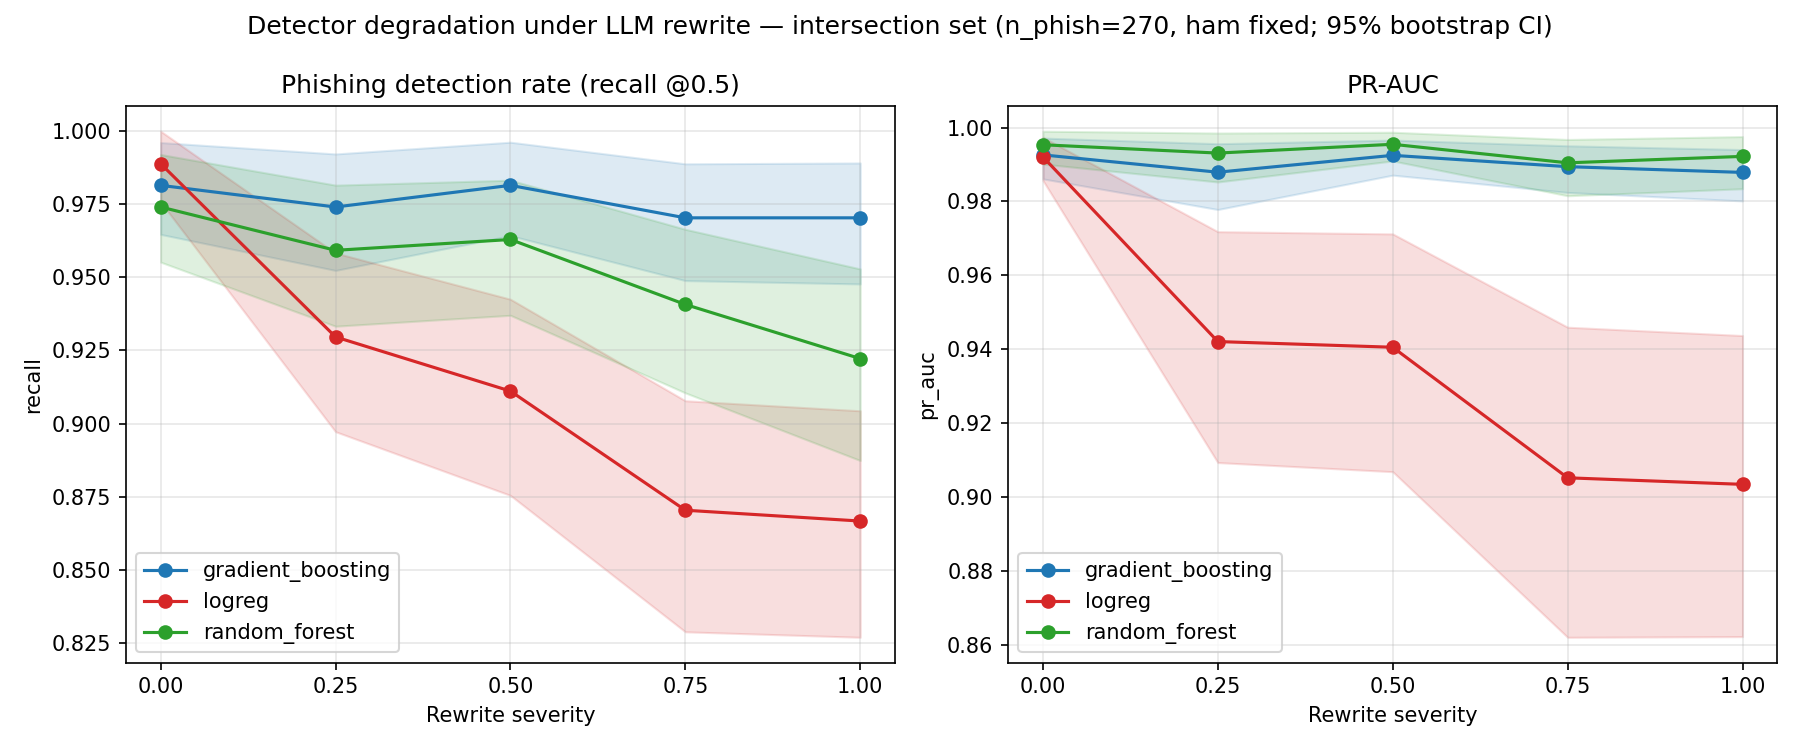
\includegraphics[width=0.92\textwidth]{figures/degradation_curve.png}
\caption{Detector degradation under LLM rewriting on the strict intersection set
($n=270$, ham fixed; 95\% bootstrap CI). Phishing detection rate (recall@0.5) and
PR-AUC versus rewrite severity. The linear model degrades most; the tree ensembles
lean on the frozen URL feature.}
\label{fig:degradation}
\end{figure}

\begin{table}[t]
\centering
\caption{URL-masked degradation, $n=270$. recall@0.5; parenthetical is the
corresponding URL-intact $\Delta$ from Table~\ref{tab:headline}.}
\label{tab:masked}
\begin{tabular}{lccr}
\toprule
model & sev 0.0 & sev 1.0 & $\Delta(0\!\to\!1)$ (vs intact) \\
\midrule
logistic regression & 0.985 & 0.763 & \dropneg{0.222}~($-0.122$) \\
random forest & 0.948 & 0.856 & $-0.093$~($-0.052$) \\
gradient boosting & 0.978 & 0.926 & $-0.052$~($-0.011$) \\
\bottomrule
\end{tabular}
\end{table}

\subsection{Significance}
A paired McNemar exact test (sev~$0.0$ vs $1.0$, strict $n=270$) confirms the
drops are not noise (Table~\ref{tab:significance}). Every URL-masked cell and all
but one URL-intact cell are significant; the lone exception is gradient boosting
with URLs intact (drop 1.1 pts, $p\approx0.58$), which barely degrades when the URL
signal is present.

\begin{table}[t]
\centering
\caption{Paired McNemar exact significance, det@0.5, sev~$0.0\!\to\!1.0$.}
\label{tab:significance}
\begin{tabular}{llrl}
\toprule
condition & model & drop (pts) & McNemar $p$ \\
\midrule
original & logistic regression & 12.2 & \num{2.10e-9} \\
original & random forest & 5.2 & \num{4.34e-3} \\
original & gradient boosting & 1.1 & \num{5.81e-1} (NS) \\
url-masked & logistic regression & 22.2 & \num{2.73e-17} \\
url-masked & random forest & 9.3 & \num{1.12e-4} \\
url-masked & gradient boosting & 5.2 & \num{9.36e-3} \\
\bottomrule
\end{tabular}
\end{table}

\subsection{Cross-model confirmation (Gemini)}
An independent rewriting model (Gemini 2.5 Flash, $n=308$) reproduces the
qualitative shape: logreg recall@0.5 falls $0.990\!\to\!0.948$
(\dropneg{0.042}), with the linear model most fragile and the trees URL-anchored.
The effect is not specific to a single attacker model; two models is confirmation,
not an exhaustive survey.

\subsection{Era ablation}
Splitting the strict set by corpus era (legacy eBay/PayPal-era mbox, $n=128$ vs
modern by-year, $n=142$) shows the attack degrades modern phishing more (logreg
\dropneg{0.190} vs \dropneg{0.047}). We read this as indicative only: the strict
checker over-fails the brand-footer-heavy legacy bucket, so the split is on a
non-random subsample (see \S\ref{sec:limitations}).

\subsection{Transformer detector: corpus-dependent robustness}
On the Nazario phishing corpus, the fine-tuned DistilBERT \emph{resists} the
attack: recall@0.5 holds at 100.0\% across all severities (drop 0.0 pts, McNemar
$p=1.0$), and it is not URL-anchored---under inference-time URL masking, recall
stays 99.6\% at sev~1.0. This is the opposite of the bag-of-words detectors.

We deliberately do \emph{not} generalise this to ``transformers are robust.'' On an
independent, same-era spam corpus (CEAS-2008, \S\ref{sec:external}) the
\emph{same} transformer degrades significantly under the same attack
(\dropneg{0.148}, $p=\num{3.9e-3}$) and \emph{is} URL-anchored there (URL-masked
drop \dropneg{0.426}). The transformer's resistance is therefore corpus-dependent;
the most we can claim is that on Nazario phishing it held where the lexical
detectors broke.

\subsection{External validity: CEAS-2008}\label{sec:external}
To remove the era confound between recent phishing and older ham, we replicate on
CEAS-2008 \citep{champa2023phishing}, where both classes are from 2008.
(CEAS labels are generic spam, not phishing specifically; this is a deliberate
generality check, surfaced as a caveat.) Both the degradation curve and the
URL-masking amplification reproduce: every original-condition drop is
McNemar-significant (logreg 23.0 pts $p=\num{1.2e-4}$; random forest 55.7 pts
$p=\num{1.2e-10}$; gradient boosting 26.2 pts $p=\num{3.1e-5}$), and URL masking
enlarges the sev-1.0 logreg drop further (roughly $0.23\!\to\!0.48$). The finding
is not a quirk of the primary dataset or of phishing-vs-spam labelling.

\section{Mitigation}\label{sec:mitigation}
\paragraph{Adversarial training.} Augmenting the training set with passing
severity-$\geq0.5$ rewrites and retraining closes the gap entirely. On the
URL-masked, sev-1.0 case---the hardest---logistic-regression recall recovers from
0.763 to 0.989, at or above its own clean baseline (0.985). The degradation is a
fixable training-distribution gap, not an inherent ceiling.

\paragraph{Cross-generator generalization.} The key test is whether recovery is
generator-specific overfitting. We score the \emph{identical} Haiku-trained
adversarial detectors against held-out \emph{Gemini} rewrites ($n=308$): every cell
shows the adversarial model $\geq$ baseline, and recovery is largest exactly where
the attack bit hardest---the URL-masked linear model, where det@1\%FPR rises
$0.890\!\to\!0.994$ (\textbf{$+0.104$}), reaching the same near-ceiling as the
Haiku-on-Haiku run. The reverse direction (train on Gemini, test on Haiku) agrees:
after Gemini-augmented training, 0 of 6 baseline-significant degradations remain
significant. Adversarial training is \textbf{generator-agnostic}---though this is
one cross-generator pair, strong evidence of transfer rather than a proof of
universality.

\section{Limitations}\label{sec:limitations}
We state the main threats to validity; several mean the reported degradation is, if
anything, an \emph{under}-estimate.
\begin{itemize}
  \item \textbf{Conservative retention checker.} The strict all-URLs contract
  discards genuinely valid rewrites that drop only incidental (footer/tracking)
  links, so the strict headline set is a lower bound on attack success.
  \item \textbf{ROC-AUC insensitivity.} Under $\sim1\!:\!4.4$ imbalance, ROC-AUC
  barely moves; we report recall@0.5, det@1\%FPR, and PR-AUC instead.
  \item \textbf{English-only, single phishing source.} All corpora are
  predominantly English; phishing positives come only from Nazario. The era
  ablation partially addresses source confounds; CEAS-2008 provides off-corpus
  external validity.
  \item \textbf{URL-frozen contract.} Freezing URLs isolates the text signal and
  keeps labels valid, but hands the defender an unperturbed feature; the URL-masked
  curve is the more realistic text-only bound.
  \item \textbf{Two rewriting models.} Haiku and Gemini confirm the effect is not
  model-specific, but are not an exhaustive survey.
\end{itemize}

\section{Ethics and Responsible Release}\label{sec:ethics}
PhishRewrite is a defensive-research artifact: the rewrites exist solely to measure
detector robustness, not as deployable evasive content. The released data is
derived entirely from public named research corpora, with all URLs defanged
(scheme-only, losslessly reversible) so the release carries no live phishing links;
no PII is collected, no email is sent, and no live infrastructure is involved.
Permitted uses are academic study, detector evaluation, and hardening; sending
email, real phishing/social-engineering, and deployment against people or live
systems are prohibited. The mitigation results (\S\ref{sec:mitigation}) show a
concrete, generator-agnostic defence, which we consider central to releasing the
attack responsibly.

\section{Conclusion}
Content-based phishing detectors are fragile under LLM rewriting that preserves the
malicious ask---most acutely for linear models, and more so once the frozen URL
signal is removed. Neural robustness, where it appears, is corpus-dependent rather
than guaranteed. Encouragingly, the gap is fixable: adversarial training on
rewrites restores and exceeds clean detection and generalizes across rewriting
model families. We release the benchmark, code, and prompts to support reproducible
detector hardening.

\paragraph{Availability.} Benchmark and code:
\url{https://github.com/gaurangkatyal/phishrewrite}; archived data at
\url{https://doi.org/10.5281/zenodo.21018699} (v1.0:
\url{https://doi.org/10.5281/zenodo.21018700}).

\bibliographystyle{plainnat}
\bibliography{references}

\end{document}
